\begin{figure}[!t]
    \resizebox{\linewidth}{!}{%

    \begin{minipage}[t]{.625\linewidth}
    \centering
    \strut\vspace*{-9mm}\newline
    
        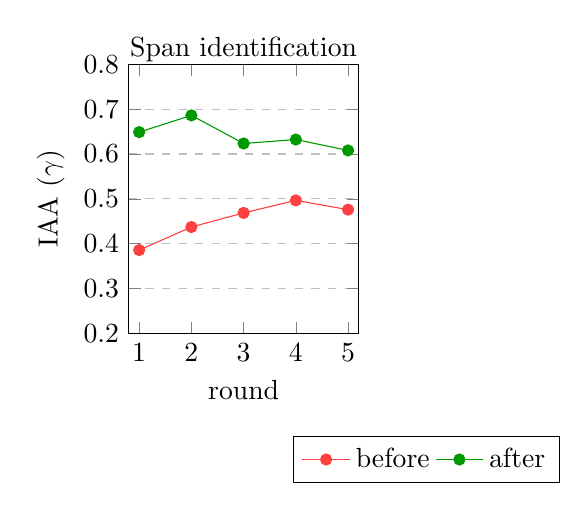
\begin{tikzpicture}
            \begin{axis}[
                xlabel={round},
                ylabel={IAA ($\gamma$)},
                xmin=0.8, xmax=5.2,
                ymin=0.2, ymax=0.8,
                xtick={1,2,3,4,5},
                ytick={0.8,0.7,0.6,0.5,0.4,0.3,0.2},
                height=5cm,
                width=4.5cm,
                legend pos=south west,
                ymajorgrids=true,
                grid style=dashed,
                title style={yshift=-3mm},
                legend style={yshift=-20mm,xshift=20mm},
                legend columns=-1,
                title={Span identification}
            ]

            \addplot[
                color=red!75!white,
                mark=*,
                ]
                coordinates {
                (1,0.3857821393988512)(2,0.4371931547450958)(3,0.4686853509164328)(4,0.49652522783298525)(5,0.4759202686989723)
                };
            \addlegendentry{before}

            \addplot[
                color=green!60!black,
                mark=*,
                ]
                coordinates {
                (1,0.6487089802126298)(2,0.6860159984821426)(3,0.6233792631234466)(4,0.6321975576824279)
                (5,0.6079000891877535)};
            \addlegendentry{after}
            \end{axis}
        \end{tikzpicture}
        
        %\\

    \end{minipage}\hfill
    \begin{minipage}[t]{.625\linewidth}
    \centering
    \strut\vspace*{-9mm}\newline
        
        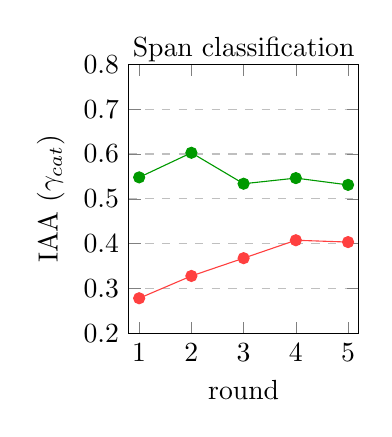
\begin{tikzpicture}
            \begin{axis}[
                xlabel={round},
                ylabel={IAA ($\gamma_{cat}$)},
                xmin=0.8, xmax=5.2,
                ymin=0.2, ymax=0.8,
                xtick={1,2,3,4,5},
                ytick={0.8,0.7,0.6,0.5,0.4,0.3,0.2},
                %yticklabel=\empty,
                height=5cm,
                width=4.5cm,
                legend pos=south west,
                ymajorgrids=true,
                grid style=dashed,
                title style={yshift=-3mm},
                legend style={yshift=-20mm, draw=none},
                title={Span classification}
            ]

            \addplot[
                color=red!75!white,
                mark=*,
                ]
                coordinates {
                (1,0.2784156236556151)(2,0.3280955837910706)(3,0.3677531504002608)(4,0.40771429851679253)(5,0.40363390145288314)
                };
            %\addlegendentry{before}
            
            \addplot[
                color=green!60!black,
                mark=*,
                ]
                coordinates {
                (1,0.5478709892625211)(2,0.6026936344138025)(3,0.5336831054261926)(4,0.5462384763261199)
                (5,0.531095305115031)};
            %\addlegendentry{after}
            \end{axis}
        \end{tikzpicture}
    
    \end{minipage}
}%
	\caption{Inter-annotator agreement (IAA) scores for both span identification ($\gamma$) and classification ($\gamma_{cat}$) at each annotation round, \emph{before} and \emph{after} discussion.}
	\label{fig:iaa}
\end{figure}